\documentclass[14pt]{extbook}
\usepackage{multicol, enumerate, enumitem, hyperref, color, soul, setspace, parskip, fancyhdr} %General Packages
\usepackage{amssymb, amsthm, amsmath, bbm, latexsym, units, mathtools} %Math Packages
\everymath{\displaystyle} %All math in Display Style
% Packages with additional options
\usepackage[headsep=0.5cm,headheight=12pt, left=1 in,right= 1 in,top= 1 in,bottom= 1 in]{geometry}
\usepackage[usenames,dvipsnames]{xcolor}
\usepackage{dashrule}  % Package to use the command below to create lines between items
\newcommand{\litem}[1]{\item#1\hspace*{-1cm}\rule{\textwidth}{0.4pt}}
\pagestyle{fancy}
\lhead{Progress Quiz 9}
\chead{}
\rhead{Version A}
\lfoot{8590-6105}
\cfoot{}
\rfoot{Fall 2020}
\begin{document}

\begin{enumerate}
\litem{
Describe the end behavior of the polynomial below.\[ f(x) = -6(x - 7)^{3}(x + 7)^{8}(x + 2)^{3}(x - 2)^{3} \]\begin{enumerate}[label=\Alph*.]
\begin{multicols}{2}\item 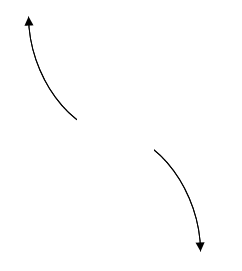
\includegraphics[width = 0.3\textwidth]{../Figures/polyEndBehaviorAA.png}\item 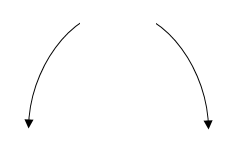
\includegraphics[width = 0.3\textwidth]{../Figures/polyEndBehaviorBA.png}\item 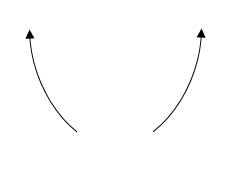
\includegraphics[width = 0.3\textwidth]{../Figures/polyEndBehaviorCA.png}\item 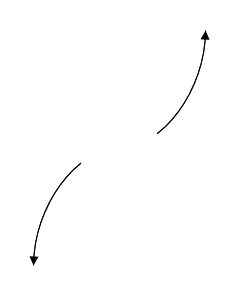
\includegraphics[width = 0.3\textwidth]{../Figures/polyEndBehaviorDA.png}\end{multicols}\item None of the above.
\end{enumerate} }
\litem{
Which of the following equations \textit{could} be of the graph presented below?
\begin{center}
    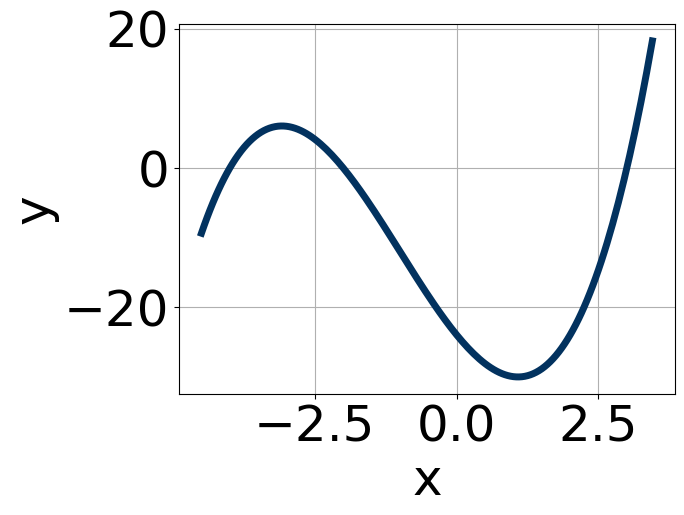
\includegraphics[width=0.5\textwidth]{../Figures/polyGraphToFunctionCopyA.png}
\end{center}
\begin{enumerate}[label=\Alph*.]
\item \( 8x^{4} (x - 1)^{4} (x + 2)^{11} \)
\item \( -15x^{4} (x - 1)^{11} (x + 2)^{10} \)
\item \( -3x^{10} (x - 1)^{9} (x + 2)^{11} \)
\item \( 16x^{8} (x - 1)^{8} (x + 2)^{4} \)
\item \( -20x^{4} (x - 1)^{6} (x + 2)^{7} \)

\end{enumerate} }
\litem{
Construct the lowest-degree polynomial given the zeros below. Then, choose the intervals that contain the coefficients of the polynomial in the form $ax^3+bx^2+cx+d$.\[ \frac{-2}{3}, \frac{4}{5}, \text{ and } \frac{-5}{4} \]\begin{enumerate}[label=\Alph*.]
\item \( a \in [51, 65], b \in [-78, -65], c \in [-43, -39], \text{ and } d \in [40, 46] \)
\item \( a \in [51, 65], b \in [64, 74], c \in [-43, -39], \text{ and } d \in [40, 46] \)
\item \( a \in [51, 65], b \in [64, 74], c \in [-43, -39], \text{ and } d \in [-41, -38] \)
\item \( a \in [51, 65], b \in [82, 84], c \in [-26, -18], \text{ and } d \in [-41, -38] \)
\item \( a \in [51, 65], b \in [-13, -11], c \in [-83, -76], \text{ and } d \in [40, 46] \)

\end{enumerate} }
\litem{
Construct the lowest-degree polynomial given the zeros below. Then, choose the intervals that contain the coefficients of the polynomial in the form $ax^3+bx^2+cx+d$.\[ 5, \frac{7}{4}, \text{ and } \frac{1}{4} \]\begin{enumerate}[label=\Alph*.]
\item \( a \in [12, 26], b \in [-113, -109], c \in [157, 171], \text{ and } d \in [-45, -34] \)
\item \( a \in [12, 26], b \in [102, 105], c \in [113, 118], \text{ and } d \in [-45, -34] \)
\item \( a \in [12, 26], b \in [48, 52], c \in [-153, -150], \text{ and } d \in [34, 42] \)
\item \( a \in [12, 26], b \in [112, 116], c \in [157, 171], \text{ and } d \in [34, 42] \)
\item \( a \in [12, 26], b \in [-113, -109], c \in [157, 171], \text{ and } d \in [34, 42] \)

\end{enumerate} }
\litem{
Construct the lowest-degree polynomial given the zeros below. Then, choose the intervals that contain the coefficients of the polynomial in the form $x^3+bx^2+cx+d$.\[ 4 - 5 i \text{ and } -2 \]\begin{enumerate}[label=\Alph*.]
\item \( b \in [0.3, 3.1], c \in [5, 10], \text{ and } d \in [8, 12] \)
\item \( b \in [2.1, 8.9], c \in [15, 28], \text{ and } d \in [-89, -71] \)
\item \( b \in [0.3, 3.1], c \in [-3, -1], \text{ and } d \in [-8, -3] \)
\item \( b \in [-7.3, -5.9], c \in [15, 28], \text{ and } d \in [82, 85] \)
\item \( \text{None of the above.} \)

\end{enumerate} }
\litem{
Construct the lowest-degree polynomial given the zeros below. Then, choose the intervals that contain the coefficients of the polynomial in the form $x^3+bx^2+cx+d$.\[ -3 - 5 i \text{ and } 3 \]\begin{enumerate}[label=\Alph*.]
\item \( b \in [-0.42, 1.63], c \in [-3.2, 1], \text{ and } d \in [-14, -6] \)
\item \( b \in [-4.7, -1.52], c \in [14.7, 18.4], \text{ and } d \in [102, 106] \)
\item \( b \in [-0.42, 1.63], c \in [1.8, 4.8], \text{ and } d \in [-17, -13] \)
\item \( b \in [2.39, 3.09], c \in [14.7, 18.4], \text{ and } d \in [-107, -92] \)
\item \( \text{None of the above.} \)

\end{enumerate} }
\litem{
Describe the zero behavior of the zero $x = -2$ of the polynomial below.\[ f(x) = -9(x - 5)^{6}(x + 5)^{5}(x - 2)^{11}(x + 2)^{6} \]\begin{enumerate}[label=\Alph*.]
\begin{multicols}{2}\item 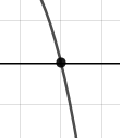
\includegraphics[width = 0.3\textwidth]{../Figures/polyZeroBehaviorCopyAA.png}\item 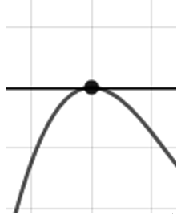
\includegraphics[width = 0.3\textwidth]{../Figures/polyZeroBehaviorCopyBA.png}\item 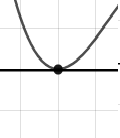
\includegraphics[width = 0.3\textwidth]{../Figures/polyZeroBehaviorCopyCA.png}\item 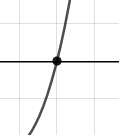
\includegraphics[width = 0.3\textwidth]{../Figures/polyZeroBehaviorCopyDA.png}\end{multicols}\item None of the above.
\end{enumerate} }
\litem{
Describe the end behavior of the polynomial below.\[ f(x) = -5(x + 8)^{2}(x - 8)^{5}(x + 7)^{3}(x - 7)^{3} \]\begin{enumerate}[label=\Alph*.]
\begin{multicols}{2}\item 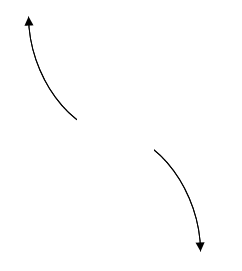
\includegraphics[width = 0.3\textwidth]{../Figures/polyEndBehaviorCopyAA.png}\item 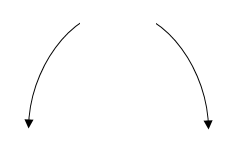
\includegraphics[width = 0.3\textwidth]{../Figures/polyEndBehaviorCopyBA.png}\item 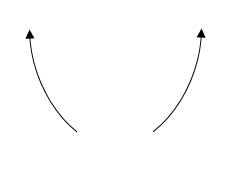
\includegraphics[width = 0.3\textwidth]{../Figures/polyEndBehaviorCopyCA.png}\item 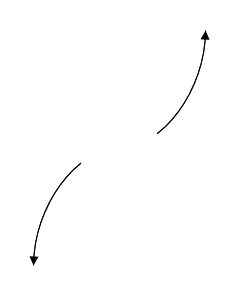
\includegraphics[width = 0.3\textwidth]{../Figures/polyEndBehaviorCopyDA.png}\end{multicols}\item None of the above.
\end{enumerate} }
\litem{
Which of the following equations \textit{could} be of the graph presented below?
\begin{center}
    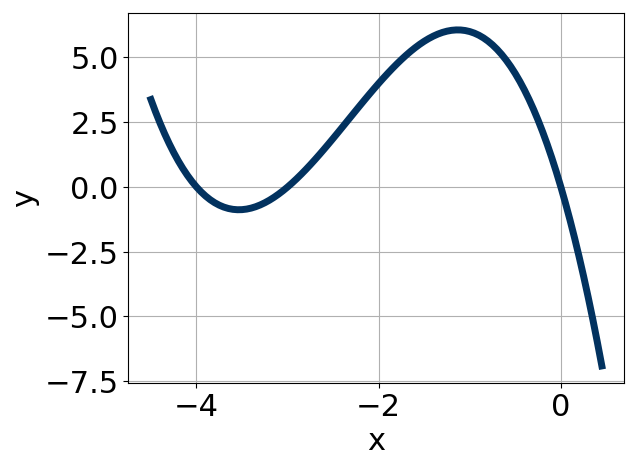
\includegraphics[width=0.5\textwidth]{../Figures/polyGraphToFunctionA.png}
\end{center}
\begin{enumerate}[label=\Alph*.]
\item \( -4(x + 4)^{9} (x + 1)^{9} (x + 2)^{5} \)
\item \( -2(x + 4)^{4} (x + 1)^{5} (x + 2)^{11} \)
\item \( 20(x + 4)^{11} (x + 1)^{7} (x + 2)^{11} \)
\item \( 10(x + 4)^{4} (x + 1)^{9} (x + 2)^{11} \)
\item \( 12(x + 4)^{10} (x + 1)^{8} (x + 2)^{7} \)

\end{enumerate} }
\litem{
Describe the zero behavior of the zero $x = 2$ of the polynomial below.\[ f(x) = -7(x + 2)^{2}(x - 2)^{7}(x + 7)^{3}(x - 7)^{4} \]\begin{enumerate}[label=\Alph*.]
\begin{multicols}{2}\item 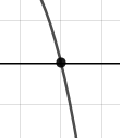
\includegraphics[width = 0.3\textwidth]{../Figures/polyZeroBehaviorAA.png}\item 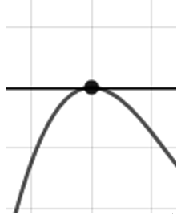
\includegraphics[width = 0.3\textwidth]{../Figures/polyZeroBehaviorBA.png}\item 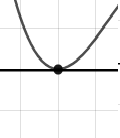
\includegraphics[width = 0.3\textwidth]{../Figures/polyZeroBehaviorCA.png}\item 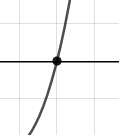
\includegraphics[width = 0.3\textwidth]{../Figures/polyZeroBehaviorDA.png}\end{multicols}\item None of the above.
\end{enumerate} }
\end{enumerate}

\end{document}